% !TEX program = xelatex
\documentclass[11pt]{beamer}

\usepackage{unicode-math}
\usepackage[style=ddmmyyyy]{datetime2}
\usepackage{graphicx}
\usepackage{hyperref}
\usepackage{fontspec}
\usepackage{xcolor}

\makeatletter
\def\input@path{{../../theme/}}
\makeatother

\usetheme{mis}

\setsansfont{Rosario}[Numbers=OldStyle]
\setmathfont{STIX Two Math}[Scale=MatchLowercase]
\setmonofont{Consolas}[Scale=MatchLowercase]

\author{Lê Thành Văn}
\title{Lập trình nâng cao}
\institute{Khoa Hệ thống thông tin quản lý}
\date{\today}
% package setting
\hypersetup {
	colorlinks = true
}
%\usecolortheme{seahorse}
% short hand
\newcommand{\pandas}{\texttt{pandas}}
%
\AtBeginSection{
  \frame{
    \sectionpage
  }
}
% graphic path
\graphicspath{{../../media/}}

\begin{document}

	\begin{frame}
		\titlepage
	\end{frame}

	\section{Giới thiệu}
	\begin{frame}{Mục đích}
		\begin{itemize}
			\item Nắm được các giai đoạn phân tích dữ liệu.
			\item Nắm và vận dụng các kỹ năng cơ bản khi phân tích dữ liệu.
			\item Nắm được các thuật toán machine learning cơ bản.
		\end{itemize}
	\end{frame}

	\begin{frame}{Nội dung}
		Môn học bao gồm 2 phần chính :
		\begin{itemize}
			\item Làm việc với \texttt{DataFrame} (thư viện \pandas\ của Python).
			\item Giới thiệu về machine learning và các thuật toán cơ bản.
		\end{itemize}
	\end{frame}

	\begin{frame}{Thời khóa biểu}
		Chương trình học gồm 15 buổi (3 tiết một buổi):
		\begin{itemize}
			\item Thứ 3 (tiết 7): 01/12/2020 -- 19/01/2021.
			\item Thứ 6 (tiết 7): 04/12/2020 -- 22/01/2021.
		\end{itemize}
	\end{frame}

	\begin{frame}{Điểm số}
		Điểm quá trình (50\%):
		\begin{itemize}
			\item Điểm chuyên cần (40\%).
			\item Điểm bài tập (60\%).
		\end{itemize}
		Điểm cuối kỳ (50\%) (thi thực hành).
	\end{frame}

	\section{Tài liệu tham khảo}
	\begin{frame}{\pandas}
		\begin{itemize}
			\item \href{https://www.tutorialspoint.com/python_pandas/index.htm}{Hướng dẫn \pandas.}
			\item \href{https://pandas.pydata.org/docs/}{\pandas ' documentation}: tài liệu của \pandas{} (phương thức, kiểu dữ liệu, ...).
			\item \href{https://stackoverflow.com/questions/tagged/pandas}{Stack Overflow về \pandas{}}: hỏi đáp về \pandas.
		\end{itemize}
	\end{frame}

	\begin{frame}{Machine Learning}
		\begin{itemize}
			\item \href{https://scikit-learn.org/stable/documentation.html}{scikit-learn's documentation} : tài liệu của scikit-learn (thư viện machine learning của microsoft)
			\item \href{https://www.tensorflow.org/tutorials/}{Hướng dẫn về TensorFlow} : thư viện machine learning của Google
		\end{itemize}
	\end{frame}

	\begin{frame}{Khóa học}
		\begin{itemize}
			\item \href{https://courses.edx.org/courses/course-v1:Microsoft+DAT210x+6T2016/course/}{Programming with Python for Data Science} : khóa học về \pandas{} và một số thuật toán cơ bản trong machine learning.
			\item \href{https://www.coursera.org/learn/machine-learning}{Khóa học machine learning của Andrew Ng}
		\end{itemize}
	\end{frame}

	\begin{frame}{Khác}
		Sách:
		\begin{itemize}
			\item \href{https://pdfs.semanticscholar.org/ce61/5ae61d67db8537e981a0a08da7f0f2ff1cee.pdf?_ga=2.176850727.342533066.1573446520-1563216005.1573446520}{Understanding Machine Learning: From Theory to Algorithms.}
			\item \href{https://www.amazon.com/Machine-Learning-Hackers-Studies-Algorithms/dp/1449303714}{Machine Learning for Hackers: Case Studies and Algorithms to Get You Started}
		\end{itemize}
		Internet:
		\begin{itemize}
			\item \href{https://machinelearningcoban.com/}{Machine Learning cơ bản}
		\end{itemize}
	\end{frame}

	\section{Thư viện \pandas}
		\begin{frame}{Giới thiệu}
			\begin{itemize}
				\item Là thư viện Python được phát triển bởi Wes McKinney từ năm 2008.
				\item Là thư viện cho việc phân tích dữ liệu khi dùng Python.
			\end{itemize}
		\end{frame}
		
		\begin{frame}{Tính năng}
			\begin{itemize}
				\item Có thể xử lý tập dữ liệu khác nhau về định dạng.
				\item Có khả năng đọc dữ liệu từ nhiều nguồn khác nhau (csv, db/sql, excel, ...).
				\item Có thể xử lý nhiều phép toán cho tập dữ liệu.
				\item Xử lý mất mát dữ liệu.
			\end{itemize}
		\end{frame}

	\begin{frame}{Các kiểu dữ liệu}
		\begin{itemize}
			\item \texttt{Series} : kiểu dữ liệu dạng mảng 1 chiều
			\item \texttt{DataFrame} : kiểu dữ liệu mảng 2 chiều
			\item \texttt{Panel} : kiểu dữ liệu mảng 3 chiều
		\end{itemize}
	\end{frame}

	\begin{frame}{Cài đặt}
		Cài đặt mới: \textcolor{red}{\texttt{pip install pandas}}.\\
		Cập nhật: \textcolor{red}{\texttt{pip install pandas --upgrade}}.
	\end{frame}

	\begin{frame}{Sử dụng}
		Người ta thường import \pandas\ như sau:\\
		\centering
		\textcolor{red}{\texttt{import pandas as pd}}
	\end{frame}

	\section{Machine Learning}
	\begin{frame}{Giới thiệu}
		Machine learning (máy học) là những phương pháp cung cấp cho máy tính cách học hỏi mà không cần hướng dẫn chi tiết từng bước.\\
		Machine learning là một lĩnh vực của Artificial Intelligence (AI, trí tuệ nhân tạo)
	\end{frame}

	\begin{frame}{Phương pháp}
	Machine learning bao gồm các phương pháp sau:
		\begin{itemize}
			\item Supervised Learning: học có giám sát (phân loại (classification), hồi quy (regression), \dots)
			\item Unsupervised Learning: học không giám sát (phân nhóm (clustering), \dots)
			\item Reinforcement Learning: học củng cố (học sâu (deep learing), mạng nơ-ron (neural networks), \dots)
		\end{itemize}
	\end{frame}

	\begin{frame}{Vấn đề giải quyết được}
		Hiện tại, có rất nhiều vấn đề được giải quyết bằng machine learning
		\begin{itemize}
			\item Xử lý ảnh (gắn thẻ hình ảnh, nhận diện ký tự, nhận diện khuôn mặt, ...)
			\item Xử lý văn bản (phát hiện spam, phân tích ngữ nghĩa, ...)
			\item Khai phá dữ liệu (gom nhóm, dự đoán, ...)
		\end{itemize}
	\end{frame}

	\begin{frame}{Quy trình cơ bản}
		Thông thường, người ta sử dụng quy trình sau để giải quyết vấn đề bằng machine learing:
		\begin{enumerate}
			\item Thu thập dữ liệu
			\item Làm sạch dữ liệu
			\item Khám phá dữ liệu
			\item Chuyển đổi dữ liệu
			\item Xây dựng mô hình
			\item Đánh giá và điều chỉnh
		\end{enumerate}
	\end{frame}

	\begin{frame}
		\begin{figure}
			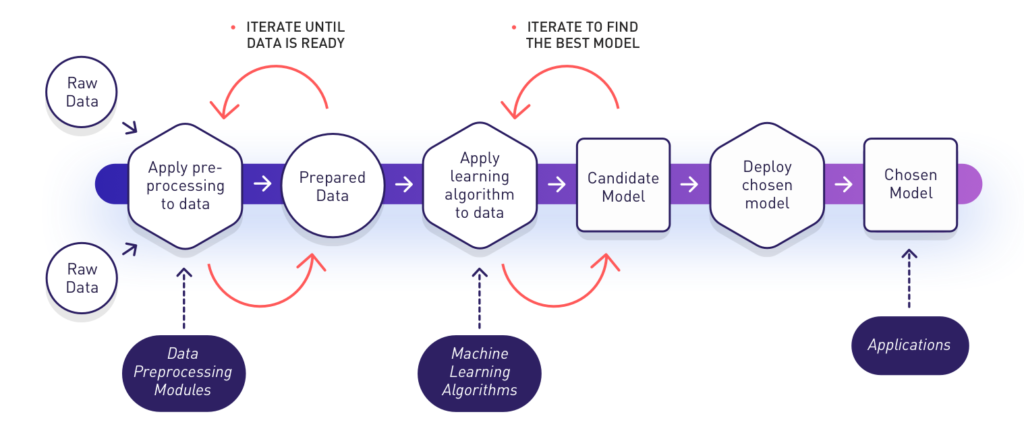
\includegraphics[width=\textwidth]{ml.png}
			\caption{Quy trình cơ bản}
		\end{figure}
	\end{frame}

	\begin{frame}{Machine learning trong Python}
		Trong python có nhiều package về machine learning như \texttt{scikit-learn}, \texttt{TensorFlow}, \dots
	\end{frame}

\end{document} 
